\documentclass[12pt,openany]{book}
\usepackage{geometry,graphicx,color}
\usepackage{fontspec}
\usepackage{emoji}
\newfontface\Emojifont{Apple Color Emoji}[Renderer=HarfBuzz]
\usepackage[nofontspec]{newpxtext}
\usepackage[dvipsnames]{xcolor}
\usepackage{mathrsfs}
\usepackage{fancyhdr}
\usepackage{mathrsfs}
\usepackage{empheq}
\usepackage{dsserif}
\usepackage{amssymb,amsmath,mathrsfs}    
\geometry{
  a4paper,
  top=25.4mm, bottom=25.4mm,
  left=20mm, right=20mm,
  headheight=2.17cm,
  headsep=4mm,
  footskip=12mm
}
\usepackage[strict]{changepage} % 提供一个 adjustwidth 环境
\usepackage{framed} % 实现方框效果
\usepackage[most]{tcolorbox}
\usepackage{mathpazo}% 采用 Palatino 风格字体
\usepackage{empheq}
\usepackage{physics}



\tcbuselibrary{breakable,theorems}

\definecolor{winered}{rgb}{0.5,0,0}
\definecolor{structurecolor}{RGB}{122,122,142}
\definecolor{main}{HTML}{3D445F}
\definecolor{second}{HTML}{627581}
\definecolor{third}{HTML}{9D8798}
\definecolor{maincolor}{RGB}{199,210,212}

% 定义引用的颜色
\usepackage{hyperref}
\hypersetup{colorlinks = true, linktoc=all, linkcolor=black, urlcolor=winered}

\newtcbox{\mymath}[1][]{
    nobeforeafter, math upper, tcbox raise base,
    enhanced, colframe=blue!30!black,
    colback=blue!30, boxrule=1pt,
    #1}


% ------------------------------------------------------------%
%%%%%%%%%%颜色设置
\definecolor{formalshade}{rgb}{0.95,0.95,1} % 文本框颜色
\definecolor{Blue}{rgb}{0,0,0.5}

%%%%%%%文本框设置
\newenvironment{formal}{%
\def\FrameCommand{%
\hspace{1pt}%
{\color{Blue}\vrule width 2pt}%
{\color{formalshade}\vrule width 4pt}%
\colorbox{formalshade}%
}%
\MakeFramed{\advance\hsize-\width\FrameRestore}%
\noindent\hspace{-4.55pt}% disable indenting first paragraph
\begin{adjustwidth}{}{7pt}%
\vspace{2pt}\vspace{2pt}%
}
{%
\vspace{2pt}\end{adjustwidth}\endMakeFramed%
}


% ---------------------------------------------------------%
% 设置章形式
\usepackage{titlesec, titletoc}
\linespread{1.2} 				
\usepackage{fancyhdr}
\fancyhf{}
\renewcommand{\headrule}{\color{structurecolor}\hrule width\textwidth}
\pagestyle{fancy}
\renewcommand{\headrulewidth}{1pt}
\fancypagestyle{plain}{\renewcommand{\headrulewidth}{0pt}\fancyhf{}\renewcommand{\headrule}{}}

\fancyhead[c]{\color{structurecolor}\rightmark}
\fancyfoot[c]{\color{structurecolor}\small\thepage}

\titleformat{\chapter}[display]{\Large}
{\color{structurecolor}\filleft
\parbox{1cm}{\vbox to 1.5cm{\vfill\hbox to 4cm{\hfill\Huge \bfseries \color{structurecolor}{Chapter} \thechapter \hfill}}}}
{1ex}
{\color{structurecolor} \titlerule[2pt]\large\bfseries \filright \vspace*{1em}}
[\vspace*{1em} {\titlerule[2pt]}]

\titleformat{\section}[frame]{\normalfont\color{structurecolor}}{\footnotesize \enspace \large \textcolor{structurecolor}{\S \,\thesection}\enspace}{6pt}{\Large\filcenter \bf }


\titleformat{\subsection}[hang]{\bfseries}{\large\bfseries\color{structurecolor}\thesubsection\enspace}{1pt}{\color{structurecolor}\large\bfseries\filright}

\titleformat{\subsubsection}[hang]{\bfseries}{\large\bfseries\color{structurecolor}\thesubsubsection\enspace}{1pt}{\color{structurecolor}\large\bfseries\filright}
% ------------------------------------------------------------%
% 设置封面
\usepackage{titling}
\renewcommand*{\maketitle}{
    \begin{titlepage}
    \newgeometry{margin = 0in}
    \parindent=0pt
    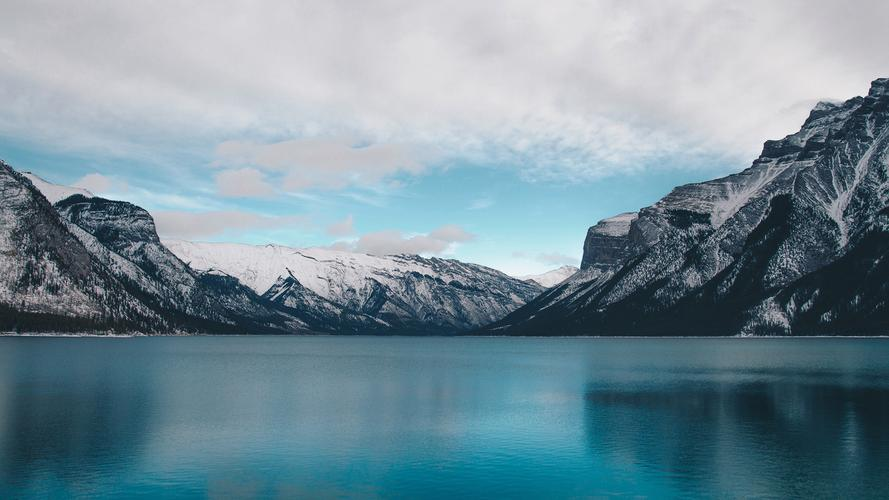
\includegraphics[width=\linewidth]{cover}
    \vfill
    \begin{center}
        \parbox{0.618\textwidth}{
        \hfill {\bfseries \Huge \thetitle} \\[0.6pt]  
        \rule{0.618\textwidth}{4pt} \\ 
    }
    \end{center}
    \vfill
    \begin{center}
        \parbox{0.618\textwidth}{
        \hfill\Large
          \begin{tabular}{r|}
          Author: \theauthor \\ 
          Date: \thedate \\
        \end{tabular}
        }
    \end{center}
    \vfill
    \begin{center}
        \parbox[t]{0.7\textwidth}{\centering }
    \end{center}
    \vfill
\end{titlepage}
\restoregeometry
\thispagestyle{empty}
}
% ------------------------------------------------------------%
\numberwithin{equation}{section}

\title{General Relativity Note}
\author{Lingyu Xia}
\date{\today}


% Define a new command for creating colored boxes with a title and text
\newcommand{\bbox}[2]{%
    \begin{tcolorbox}[title=\textbf{#1},colback=SeaGreen!10!CornflowerBlue!10,colframe=RoyalPurple!55!Aquamarine!100!]
        #2
    \end{tcolorbox}%
}

\begin{document}
\frontmatter

\maketitle
\setcounter{page}{0}
\tableofcontents

\mainmatter
\pagenumbering{arabic}
\chapter{Decay Rate \& Cross Sections}


\section{Fermi Golden Rule}

Consider time-dependent Schrödinger equation,
\begin{align}
    i\frac{d \psi}{d t}=\hat{H}(t)\psi.\label{eq:Schrödinger}
\end{align}
We can separate Hamiltonian operator into two parts, one is time-independent, and else is time-dependent,
\begin{align}
    \hat{H}(t)=\hat{H}_{0}+\hat{H^{\prime}}(\mathrm{x},t)
\end{align}
For time-independent part we can use common method to solve it,
\begin{align}
    \hat{H}_{0}\psi_{k}=E_{k}\psi_{k},\quad \text{and} \quad \braket{\psi_{j}}{\psi_{k}}=\delta_{jk}
\end{align}
Then the wavefunction can be expressed in terms of complete set of states of the unperturbed Hamiltonian as
\begin{align}
    \psi(\mathrm{x},t)=\sum_{k}c_{k}(t)\psi(\mathrm{x})e^{-i E_{k}t}.\label{eq:set1}
\end{align}

Then we can substitute Eq. \ref{eq:set1} into Eq. \ref{eq:Schrödinger}, we can get 
\begin{align}
    i \sum_k\left[\frac{\mathrm{d} c_k}{\mathrm{~d} t} \psi_k e^{-i E_k t}-i E_k c_k \psi_k e^{-i E_k t}\right] & =\sum_k c_k \hat{H}_0 \psi_k e^{-i E_k t}+\sum_k \hat{H}^{\prime} c_k \psi_k e^{-i E_k t} \notag\\
    \Rightarrow \quad i \sum_k \frac{\mathrm{d} c_k}{\mathrm{~d} t} \psi_k e^{-i E_k t} & =\sum_k \hat{H}^{\prime} c_k(t) \psi_k e^{-i E_k t}\label{eq:set2}
\end{align}
Suppose the initial state is $i$ for $\psi_{i}\equiv \ket{i}$, that is 
\begin{align}
    \psi(\mathrm{x},0)=\sum_{k}c_{k}(0)\psi_{k}=c_{i}(0)\psi_{i}.
\end{align}
We can easily imply that $c_{k}=\delta_{ik}$. Assume that time-dependent Hamiltonian is perturbed, which implies $c_{i\neq k}\ll 1, c_{i}\sim 1$. And Eq. \ref{eq:set2} can reduce to 
\begin{align}
    i \sum_k \frac{\mathrm{d} c_k}{\mathrm{~d} t} \ket{k} e^{-i E_k t} \approx \hat{H}^{\prime} \ket{i} e^{-i E_i t}\label{eq:perturbed}
\end{align}

Then we need to get to final state, so we can use relation of inner product, let $\bra{f}$ act on Eq. \ref{eq:perturbed}, we can get the coefficient $c_{f}$
\begin{align}
    \frac{d c_{f}}{dt}=-i\matrixel{f}{\hat{H'}}{i}e^{-i(E_{i}-E_{f})t},\label{eq:one_order}
\end{align}
where $\matrixel{f}{\hat{H'}}{i}\equiv T_{fi}$ is \textbf{transition matrix element}, can be calculated by
\begin{align}
    \matrixel{f}{\hat{H'}}{i}=\int_{V}\psi^{*}_{f}(\mathrm{x})\hat{H'}\psi_{i}(\mathrm{x})\dd[3]{\mathrm{x}}.
\end{align}
Then we can calculate the coefficient $c_{f}$, at time $t=T$
\begin{align}
    c_{f}(T)=-i\int^{T}_{0}T_{fi}e^{-i(E_{i}-E_{f})t}\dd{t}
\end{align}

The probability for a transition to the state $\ket{f}$ is given by
\begin{align}
    P_{if}=c_{f}^{*}(t)c_{f}(t)=\abs{T_{fi}}^{2}\int^{T}_0\int^{T}_0 e^{-i(E_{i}-E_{f})t}e^{-i(E_{i}-E_{f})t'}\dd{t}\dd{t'}
\end{align}

And we have \textbf{transition rate} $\dd{\Gamma_{fi}}$ from the initial state $\ket{i}$ to the single final state $\ket{f}$ 
\begin{align}
    \dd{\Gamma_{fi}}=\frac{P_{fi}}{T}=\frac{1}{T}\abs{T_{fi}}^{2}\int^{\frac{T}{2}}_{-\frac{T}{2}}\int^{\frac{T}{2}}_{-\frac{T}{2}} e^{-i(E_{i}-E_{f})t}e^{-i(E_{i}-E_{f})t'}\dd{t}\dd{t'}
\end{align}

If we consider the time is long enough comparing to transition process, we can take a limit,
\begin{align}
    \mathrm{d} \Gamma_{f i}=\left|T_{f i}\right|^2 \lim _{T \rightarrow \infty}\left\{\frac{1}{T} \int_{-\frac{T}{2}}^{+\frac{T}{2}} \int_{-\frac{T}{2}}^{+\frac{T}{2}} e^{i\left(E_f-E_i\right) t} e^{-i\left(E_f-E_i\right) t^{\prime}} \mathrm{d} t \mathrm{~d} t^{\prime}\right\}.
\end{align}
Associated with the definition of Dirac delta-function, the integral over $\dd t'$ can be replaced by $2\pi \delta(E_{f} -E_{i})$ and thus
\begin{align}
    \Gamma_{f i}  =2 \pi\left|T_{f i}\right|^2\left|\frac{\mathrm{d} n}{\mathrm{~d} E_f}\right|_{E_i},
\end{align}
where $\left|\frac{\mathrm{d} n}{\mathrm{~d} E_f}\right|_{E_i}$ is called \textbf{density of states}, it can be also written as 
\begin{align}
    \rho(E_{i})=\left|\frac{\mathrm{d} n}{\mathrm{~d} E_f}\right|_{E_i}
\end{align}

\textbf{Fermi's golden rule} for the total transition rate is therefore
\begin{align}
    \Gamma_{fi}=2\pi \left|T_{f i}\right|^2 \rho(E_{i})
\end{align}

However, we take assumption $c_{i\neq f}(t)\approx 0$, if we need to get more precise information, we should expand more terms of transition matrix element, we start from Eq. \ref{eq:one_order}
\begin{align}
    \frac{\mathrm{d} c_f}{\mathrm{~d} t} \approx-i\langle f|\hat{H}| i\rangle e^{i\left(E_f-E_i\right) t}+(-i)^2 \sum_{k \neq i}\left\langle f\left|\hat{H}^{\prime}\right| k\right\rangle e^{i\left(E_f-E_k\right) t} \int_0^t\left\langle k\left|\hat{H}^{\prime}\right| i\right\rangle e^{i\left(E_k-E_i\right) t^{\prime}} \mathrm{d} t^{\prime}
\end{align}
Therefore, the improved approximation for the evolution of the coefficients $c_{f}(t)$ is given by
\begin{align}
    \frac{\mathrm{d} c_f}{\mathrm{~d} t}=-i\left(\langle f|\hat{H}| i\rangle+\sum_{k \neq i} \frac{\left\langle f\left|\hat{H}^{\prime}\right| k\right\rangle\left\langle k\left|\hat{H}^{\prime}\right| i\right\rangle}{E_i-E_k}\right) e^{i\left(E_f-E_i\right) t}.
\end{align}
For second order of transition matrix element, we have 
\begin{align}
    T_{fi}=\matrixel{f}{\hat{H}}{i}+\sum_{k \neq i} \frac{\left\langle f\left|\hat{H}^{\prime}\right| k\right\rangle\left\langle k\left|\hat{H}^{\prime}\right| i\right\rangle}{E_i-E_k}
\end{align}

\section{Decay Rate}

Fermi's golden rule can be written as an alternative forma
\begin{align}
    \Gamma_{fi}=2\pi\int\abs{T_{fi}}^{2}\delta(E_{i}-E)\dd{n}\label{eq:fermi2}
\end{align}

Firstly consider the decay rate for the process $a\rightarrow 1+2$ in non-relativistic situation, related Fermi's golden rule, we write transition matrix element 
\begin{align}
    T_{fi}&=\matrixel{\psi_{1}\psi_{2}}{\hat{H'}}{\psi_{a}}\\
    &=\int_{V}\psi^{*}_1 \psi^{*}_2\hat{H'}\psi_{a}\dd[3]{x}
\end{align}

In the Born approximation, the perturbation is taken to be small and the initial- and final-state particles are represented by plane waves of the form
\begin{align}
    \psi(\mathrm{x},t)=Ae^{i(\mathbf{p}\cdot \mathrm{x}-Et)},
\end{align}
where $A^{2}=\frac{1}{V}$ determines wavefunction normalization. We use such condition
\begin{align}
    \psi(x+a,y,z)=\psi(x,y,z),\quad \text{etc.},
\end{align}
The periodic boundary conditions on the wavefunction imply that the components of momentum are quantised to
\begin{align}
    (p_{x},p_{y},p_{z})=(n_{x},n_{y},n_{z})\frac{2\pi}{a}
\end{align}

Therefore, we can get the density of states,
\begin{align}
    \dd{n}=\dd{V(p)}\frac{V}{(2\pi)^{3}}=4\pi p^{2}\dd{p}\frac{V}{(2\pi)^{3}}
\end{align}
The density of states in Fermi’s golden rule then can be obtained from
\begin{align}
    \rho(E)=\frac{\dd{n}}{\dd{E}}=\frac{\dd{n}}{\dd{p}}\abs{\frac{\dd{p}}{\dd{E}}}
\end{align}

\subsection{Lorentz-invariant Form}

To keep wavefunction normalized, a unit volume should decrease with particle energy $E=\gamma m$ increasing. For convenience, we usually take $2E$ as normalization volume
\begin{align}
    \int_{V}\psi'^{*}\psi'\dd[3]{x}=2E,
\end{align}
and therefore
\begin{align}
    \psi'=\sqrt{2E}\psi.
\end{align}

Therefore, we can get Lorentz-invariant form of transition matrix element
\begin{align}
    \mathcal{M}_{fi}=\matrixel{\psi'_{1}\psi'_{2}\cdots }{\hat{H'}}{\psi'_{a}\psi'_{b}\cdots }=\sqrt{2E_{1}\cdot 2E_{2}\cdot \cdots 2E_{a}\cdot 2E_{b}\cdots }T_{fi}
\end{align}

We go back to Fermi's golden rule. Combining with Eq. \ref{eq:fermi2}, we can get 
\begin{align}
    \Gamma_{f i}=\frac{(2 \pi)^4}{2 E_a} \int\left|\mathcal{M}_{f i}\right|^2 \delta\left(E_a-E_1-E_2\right) \delta^3\left(\mathbf{p}_a-\mathbf{p}_1-\mathbf{p}_2\right) \frac{\mathrm{d}^3 \mathbf{p}_1}{(2 \pi)^3 2 E_1} \frac{\mathrm{d}^3 \mathbf{p}_2}{(2 \pi)^3 2 E_2}.
\end{align}
It should be noticed that $\frac{\dd[3]{\mathbf{p_{i}}}}{E_{i}}$ is Lorentz-invariant.

\subsection{N-body Decay}

For N-body decay, we should generalize phase space, and the element of phase space can be expressed by 
\begin{align}
    dV_{LIPS}=\prod^{N}_{i=1} \frac{\dd[3]{\mathbf{p}_{i}}}{(2\pi)^{3}2 E_{i}},
\end{align}
where LIPS is known as Lorentz-invariant phase space.

With the definition of Dirac-delta function, we can imply that
\begin{align}
    \int \delta(E^{2}_{i}-\mathbf{p}^{2}_{i}-m^{2})\dd E_{i}=\frac{1}{E_{i}}.
\end{align}
So, we have
\begin{align}
    \int \cdots dV_{LIPS}=\int \cdots \prod_{i=1}^{N}(2\pi)^{-3}\delta(E^{2}_{i}-\mathbf{p}^{2}_i-m^{2}_i)\dd[3]{\mathbf{p}_{i}}\dd E_{i}
\end{align}

Therefore, we can write element for $a\rightarrow 1+2$ decay 
\begin{align}
    \Gamma_{fi}=\frac{(2\pi)^{4}}{2E_{a}}\int (2\pi)^{-6}\abs{\mathcal{M}_{fi}}^{2}\delta^{4}(p_{a} -p_{a}-p_{2})\delta(p^{2}_{1}-m^{2}_{1})\delta(p^{2}_{2}-m^{2}_{2})\dd[4]{p_{1}}\dd[4]{p_{2}}
\end{align}




\section{Cross-Sections}
\newpage

\mainmatter
\pagenumbering{arabic}
\chapter{Special Relativity and Classical Field Theory}

\section{Review of Special Relativity}

\subsection{Transformation}

If we have two frames of space $\mathcal{O} $ and $\mathcal{O} ^{'}$ with velocity $v$ and $u$ respectively, we want to change frame from $\mathcal{O}$ to $\mathcal{O}'$. How can we do it? For classical physics, we usually use Galilee Transformation:
\begin{align}
    \vec{u}'=\vec{u}+\vec{v}
\end{align}

But we also have to face some questions from new phenomena

\begin{itemize}
    \item What is an initial frame?
    \item It should be tested in high speed situation ($v\sim c$)
\end{itemize}

But for Lorentz transformation:

\begin{align}
    -(\delta \tau)^{2}=-(\delta t)^{2}+\frac{(\delta l)^{2}}{c^{2}}
\end{align}


\subsection{Physics in flat space: Special Relativity}

\begin{tcolorbox}[title=\textbf{Special Relativity},colback=SeaGreen!10!CornflowerBlue!10,colframe=RoyalPurple!55!Aquamarine!100!]
    The laws of nature are invariant in all inertial reference frames.

    Speed of light $c$ is constant.
\end{tcolorbox}


\bbox{Spacetime interval}{
    \begin{align}
        (\text{Interval})^{2}=(\delta s)^{2}=x^{2}+y^{2}+z^{2}-c^{2}t^{2}
    \end{align}
}

We introduce the four dimensional coordinate $x^{\mu}$

\begin{align}
    x^{\mu}=\begin{pmatrix}
    x^{0}\\
    x^{1}\\
    x^{2}\\
    x^{3}
    \end{pmatrix}=\begin{pmatrix}
    ct\\
    x\\
    y\\
    z
    \end{pmatrix}=\begin{pmatrix}
    ct\\
    x^{i}
    \end{pmatrix}
\end{align}

And metric is defined by

\begin{align}
    \eta_{\mu \nu}=\begin{pmatrix}
    -1 &  &  & \\
     & 1 &  & \\
     &  & 1 & \\
     &  &  & 1
    \end{pmatrix}_{GR}=-(\eta_{\mu\nu})_{QFT}
\end{align}

So the interval can be calculated by a metric and two four dimensional vectors

\begin{align}
    \Delta s^{2}=\begin{pmatrix}
    x^{0} &x^{1}  &x^{2}  &x^{3} 
    \end{pmatrix} \begin{pmatrix}
    -1 &  &  & \\
     & 1 &  & \\
     &  & 1 & \\
     &  &  & 1
    \end{pmatrix} \begin{pmatrix}
    x^{0}\\
    x^{1}\\
    x^{2}\\
    x^{3}
    \end{pmatrix}=\sum_{i=0}^{3}\eta_{\mu\nu}x^{\mu}x^{\nu}=x^{2}+y^{2}+z^{2}-c^{2}t^{2}
\end{align}

What are all the transformation which conserve the interval. For spatial rotations

\begin{align}
    R_{x}=\begin{pmatrix}
    1 &  &  & \\
     &  1&  & \\
     &  & \cos\theta &\sin \theta \\
     &  & \sin\theta &\cos\theta 
    \end{pmatrix}
\end{align}

But for Lorentz transformation, which is called "boost"

\begin{align}
    &x^{\mu'}=\Lambda^{\mu'}_{\nu}x^{\nu}\\
    &\Lambda^{\mu'}_\nu=\begin{pmatrix}
    \cosh \omega & -\sinh \omega &  & \\
    -\sinh \omega &\sinh \omega  &  & \\
     &  & 1 & \\
     &  &  & 1
    \end{pmatrix}
\end{align}

So we can prove that interval is Lorentz invariant:
\begin{align}
    \begin{aligned}
        \Delta s^{2}&=\eta_{\mu\nu}'\Delta x^{\mu'}x^{\nu'}\\
        &=\eta_{\mu\nu}'\Lambda^{\mu'}_\sigma \Delta x^{\sigma}\Lambda^{\nu'}_{\kappa} \Delta x^{\kappa}\\
        &=\eta_{\sigma \kappa}\Delta x^{\sigma}\Delta x^{\kappa}
    \end{aligned}
\end{align}

For two definitions which are covariant vectors and contravariant vectors are
\begin{itemize}
    \item Covariant vector: transformed as basis.
    \item Contravariant vector: transformed opposite to the basis like: $x^{\mu}, p^{\mu}$.
\end{itemize} 

\bbox{Proper time $\tau$}{The time as measured by an observer comoving with the clock. That doesn't see the clock moving with respect to it.}


\begin{align}
    \eta_{\mu\nu} V^{\mu}V^{\nu}=\begin{cases}
        <0,\; \text{timelike}\\
        =0,\; \text{null/lightlike}\\
        >0,\; \text{spcaelike}
    \end{cases}
\end{align}


\subsection{Special Relativity Kinematics}

\subsection{Maxwell Equation}

We have learned that Maxwell equations before

\begin{align}
    \begin{aligned}
        \nabla \cdot E &=\frac{\rho}{\epsilon_{0}}\\
        \nabla\cdot B&=0\\
        \nabla \times E&=-\frac{\partial B}{\partial t}\\
        \nabla \times B&=\mu_{0}j+\mu_{0}\epsilon_{0}\frac{\partial E}{\partial t}
    \end{aligned}
\end{align}

Use Einstein convention, we can express

\begin{align}
    \begin{aligned}
        \epsilon^{ijk}\partial_{i}B_{k}-\partial_{0}E^{i}&=4\pi J^{i}\\
        \partial_{i}E^{i}&=4\pi J^{0}\\
        \epsilon^{ijk}\partial_{j}E_{k}+\partial_{0}B^{i}&=0\\
        \partial_{i}B^{i}&=0
    \end{aligned}
\end{align}

Then we try to construct electromagnetic field tensor

\begin{align}
    F^{\mu\nu}=\begin{pmatrix}
    0 & -E_{1} &-E_{2}  &-E_{3} \\
    E_{1} & 0 & B_{3} & -B_{2}\\
    E_{2} & -B_{3} &  0& B_{1}\\
    E_{3} & B_{2} & -B_{1} &0 
    \end{pmatrix}=-F_{\mu\nu}
\end{align}

From components, we have 

\begin{align}
    \partial_{\nu}F^{\mu\nu}=4\pi J^{\mu}
\end{align}

\section{Classical Field Theory}





\newpage

\mainmatter
\pagenumbering{arabic}
\chapter{Introduction to Curved World}


\section{The principle of equivalence and its consequences}

Gravity = Geometry
\begin{itemize}
    \item How does the existence of matter / energy act to curve spacetime? - Einstein equation
    \item How do particles (including mass-less particles) travel in curved space-time, such that we call their trajectories being influenced by gravity?
\end{itemize}

Eötvös experiment :$m_{I}=m_{G}$, which implies \textbf{weak equivalence principle}.


\bbox{Strong equivalence principle}{
    At every point in arbitrary gravitational field, it is possible to choose a locally inertial coordinate system, such that (within a sufficiently small region) the laws of nature take the same form as in the unaccelerated Cartesian coordinate system
}

The action of gravity should be attributed to the curvature of space-time. No such thing as "global inertial frame". We focus on local inertial frames.

\section{Gravitational Redshift}

Because of the acceleration, Benny receives the signals when he is moving at a faster ray then when they were emitted.

For Benny position: $\begin{cases}z_{B}=\frac{1}{2}gt^{2}\\z_{A}=\frac{1}{2}gt^{2}+h\end{cases}$, and the time interval is $t_{1}=h-\frac{1}{2}gt_{1}^2$ 


A light wave at frequency $\nu$, $\nu \varpropto \Delta \tau^{-1}$. If light is emitted at freq. $v\nu_{*}$(forme the surface of star)

\begin{align}
    \nu_{*}=\nu(1-\frac{GM}{Rc^{2}})=\nu(1-\frac{\Delta \phi}{c^{2}})
\end{align}

\section{Mathematical description of curved space-time}

$\Delta \tau_{A} \neq \Delta \tau_{B} \implies $ space-time is curved in the presence of gravity. 

For equivalence principle: in a small enough region of space-time, the laws of physics are the same as in S.R.. Freely falling coordinate system :$\phi^{\alpha}$

The proper time: 
\begin{align}
    d\tau^{2}=-\frac{1}{c^{2}}\eta_{\alpha \beta}\dd{\xi^{\alpha}} \dd{\xi^{\beta}}
\end{align}

Freely falling particle:
\begin{align}
    \frac{\dd{U^{\alpha}}}{\dd{\tau}}=\frac{\dd[2]{\xi^{\alpha}}}{\dd{\tau}^{2}}=0
\end{align}

Express the proper time in arbitrary coordinate system $x^{\mu}$, for chain rule
\begin{align}
    \dd\tau^{2}&=-\frac{1}{c^{2}}\eta_{\alpha \beta}\left(\frac{\partial \xi^{\alpha}}{\partial x^{\mu}}\right)\dd{x^{\mu}} \left(\frac{\partial \xi^{\beta}}{\partial x^{\nu}}\right)\dd{x^{\nu}}\\
    &=-\frac{1}{c^{2}}\equiv \eta_{\alpha\beta}\left(\frac{\partial \xi^{\alpha}}{\partial x^{\mu}}\right)\left(\frac{\partial \xi^{\beta}}{\partial x^{\nu}}\right)
\end{align}

Then we can define the metric for arbitrary coordinate system:
\begin{align}
    g_{\mu\nu}\equiv \eta_{\mu\nu}\left(\frac{\partial \xi^{\alpha}}{\partial x^{\mu}}\right)\left(\frac{\partial \xi^{\beta}}{\partial x^{\nu}}\right)
\end{align}

In arbitrary coordinate system, a free-falling particle does same accelerate,
\begin{align}
    0&=\frac{\dd{U^{\alpha}}}{\dd{\tau}}=\frac{\dd}{\dd\tau}\left(\frac{\partial \xi^{\alpha}}{\partial x^{\mu}}\frac{\partial x^{\mu}}{\partial \tau}\right)\\
    0&=\left[\left(\frac{\partial ^{2}\xi^{\alpha}}{\partial x^{\mu}\partial x^{\nu}}\right)\left(\frac{\dd x^{\nu}}{\dd \tau}\right)\right]\frac{\dd x^{\mu}}{\dd\tau}+\left(\frac{\partial \xi^{\alpha}}{\partial x^{\mu}}\right)\left(\frac{\dd[2]{x^{\mu}}}{\dd\tau^{2}}\right)\\
    0&=\frac{\dd[2]{x^{\lambda}}}{\dd\tau}+\Gamma^{\lambda}_{\mu\nu}\frac{\dd{x^{\mu}}}{\dd\tau}\frac{x^{\nu}}{\dd\tau},
\end{align}
where $\Gamma^{\lambda}_{\mu\nu}$ is called \textbf{Affine connection}
\begin{align}
    \Gamma^{\lambda}_{\mu\nu}\equiv \frac{\partial x^{\lambda}}{\partial \xi^{\alpha}}\frac{\partial^{2}\xi^{\alpha}}{\partial x^{\mu}\partial ^{\nu}}
\end{align}

Then we can get \textbf{geodesic equation}

\begin{align}
    \frac{\dd U^{\lambda}}{\dd\tau}=-\Gamma^{\lambda}_{\mu\nu} U^{\mu}U^{\nu}
\end{align}

Then we want to find the connection between the Affine connection and the metric tensor

\begin{align}
    \frac{\partial g_{\mu\nu}}{\partial x^{\mu}}=\frac{\partial ^{2}\xi^{\alpha}}{\partial x^{\mu}\partial x^{\nu}}\eta_{\alpha\beta}+\frac{\partial \xi^{\alpha}}{\partial x^{\mu}}\frac{\partial^{2}\xi^{\beta}}{\partial x^{\nu}\partial x^{\lambda}}\eta_{\alpha \beta}
\end{align}
use $\frac{\partial^{2} \xi ^{\beta}}{\partial x^{\nu}\partial x^{\lambda}}=\Gamma^{\rho}_{\nu\lambda}\frac{\partial \xi^{\beta}}{\partial x^{\rho}}$
 
\begin{align}
    \frac{\partial g_{\mu\nu}}{\partial x^{\lambda}}=\Gamma^{\rho}_{\mu\lambda}\frac{\partial \xi^{\alpha}}{\partial x^{\rho}}\frac{\partial \xi^{\beta}}{\partial x^{\nu}}\eta_{\alpha\beta}+\Gamma^{\rho}_{\nu\lambda}\frac{\partial \xi^{\alpha}}{\partial x^{\mu}}\frac{\partial \xi^{\beta}}{\partial x^{\rho}}\eta_{\alpha \beta}=\Gamma^{\rho}_{\lambda\mu}g_{\rho\nu}+\Gamma^{\rho}_{\lambda\nu}g_{\rho\mu}
\end{align}

Integrate them, we can get the expression of Affine connection in terms of metric
\begin{align}
    \Gamma^{\sigma}_{\lambda\mu}=\frac{1}{2}g^{\nu \sigma}\left(\frac{\partial g_{\mu\nu}}{\partial x^{\lambda}}+\frac{\partial g_{\lambda \nu}}{\partial x^{\mu}}-\frac{\partial g_{\mu\lambda}}{\partial x^{\nu}}\right)
\end{align}

\bbox{Example in 2d flat space in $(r,\theta)$ coordinate}{
    \begin{align}
        &g_{\mu\nu}=\begin{pmatrix}
        1 & 0\\
        0 & r^{2}
        \end{pmatrix}\\
        &\Gamma^{r}_{\theta\theta}=-r\\
        &\Gamma^{\theta}_{r\theta}=\Gamma^{\theta}_{\theta r}=\frac{1}{r}
    \end{align}
}


\section{Parallel Transport}

\begin{align}
    \left(\frac{D v}{\dd \lambda}\right)^{\mu}\equiv \left(\frac{D v}{D \lambda}\right)^{\mu}=\frac{\dd x^{\sigma}}{\dd{x}}\nabla_{\sigma}v^{\mu}=0
\end{align}

We define Riemann tensor
\begin{align}
    {R^{\rho}}_{\sigma\mu\nu}=\partial _{\mu} \Gamma^{\rho}_{\nu\sigma}-\partial_{\nu}\Gamma^{\rho} _{\mu \sigma}+\Gamma^{\rho}_{\mu\lambda}\Gamma^{\lambda} _{\nu \sigma}-\Gamma^{\rho}_{\nu\lambda} \Gamma^{\lambda} _{\mu \sigma}
\end{align}

It follows several properties
\begin{align}
    \begin{cases}
        R_{\rho\sigma\mu\nu}=R_{\mu\nu\rho \sigma}\\
        R_{\rho \sigma \mu\nu}=-R_{\sigma\rho\mu\nu}\\
        R_{[\rho\sigma\mu\nu]}=0\\
        R^{\rho}_{\sigma(\nu \rho)}=0
    \end{cases}
\end{align}

Ricci tensor and Ricci scalar
\begin{align}
    &R_{\mu\nu}=R^{\lambda}_{\mu\lambda \nu}\\
    &R=R^{\mu}_\mu=g^{\mu\nu}R_{\mu\nu}
\end{align}

How many independent components does the Riemann tensor have?

\begin{align}
    &R_{[\mu\nu][\rho\sigma]}\rightarrow \frac{1}{2}\left[\frac{m(m+1)}{2}\right]\left[\frac{n(n-1)}{2}+1\right]\\
    &R_{[\rho\sigma\mu\nu]}\rightarrow\frac{1}{4!}n(n-1)(n-2)(n-3)
\end{align}

Bianchi indentity
\begin{align}
    \nabla_{\lambda}R_{\rho\sigma\mu\nu}&=\partial_{\lambda}R_{\rho\sigma\mu\nu}\\
    &=\frac{1}{2 }\partial_{\lambda}\left(\partial_{\mu}\partial_{\sigma}g_{\mu\nu}-\partial_{\mu}\partial_{\rho}g_{\nu\sigma}-\partial_{\nu}\partial_{\sigma}g_{\rho\mu}+\partial_{\nu}\partial_{\rho }g_{\mu\sigma}\right)
\end{align}

Also, we have
\begin{align}
    &\nabla_{\lambda}R_{\rho\sigma\mu\nu}+\nabla_{\rho}R_{\sigma\lambda\mu\nu}+\nabla_{\sigma}R_{\lambda\rho \mu\nu}=0\\
    \implies& \nabla_{[\lambda}R_{\rho\sigma]\mu\nu}=0\\
    \implies&0=\nabla^{\mu}R_{\rho\mu}-\nabla_{\rho}R+\nabla^{\mu}R_{\rho\mu}\\
    \implies&\nabla^{\mu}R_{\rho\mu}=\frac{1}{2}\nabla_{\rho}R
\end{align}

We can also derive the Einstein tensor
\begin{align}
    &G_{\mu\nu}=R_{\mu\nu}-\frac{1}{2}Rg_{\mu\nu}\\
    \implies&\nabla^{\mu}G_{\mu\nu}=0
\end{align}

\section{Einstein Equation}





\end{document}